
	
This section talks about commercial magnetostrictive materials, what alternatives are available, why we study them, and what we can do with them. 

\begin{figure}[h] 
	\centering
	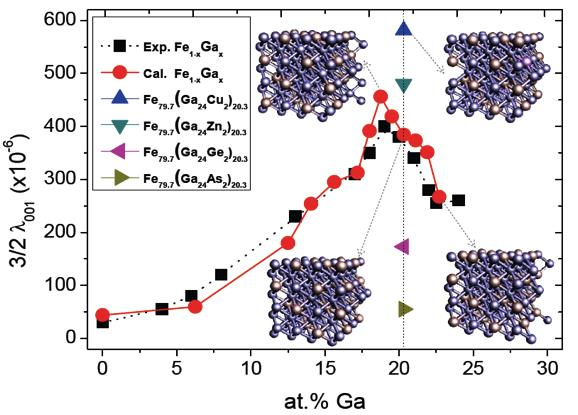
\includegraphics[trim=0pt 10pt 0pt 0pt,scale=1.5]{galfenol-composition-constant}
	\caption{Calculated tetragonal magnetostriction constant (3/2)$\lambda_{001}$ (red circles) and experimental data taken at room temperature (black squares at different Ga concentrations). Triangles show results of four ternary alloys with addition of Cu, Zn, Ge and As. %Insets give the crystal structures with purple and red balls for Fe and Ga atoms, respectively.%
	}
	\label{fig:galfenol-composition-constant}		
\end{figure}

Magnetostriction \cite{Ueno2015a} is the structural response of magnetic materials to an external magnetic field, which arises due to the dependence of the magnetocrystalline anisotropy energy on strain. The magnetostrictive coefficient $\lambda$, which is the ratio of the magnetoelastic coupling b to the shear modulus ($\lambda = b/C'$), serves as a figure of merit for magnetostrictive performance. Magnetostriction in Terfenol-D can be traced back to the strong spin-orbit (magnetoelastic) coupling of the lattice to the anisotropic electron cloud surrounding the Tb ion. The understanding of magnetostriction in Galfenol is more challenging, because spin-orbit coupling is generally weaker in the 3\textit{d} transition metals and the electron cloud surrounding the Fe ion is more deformable than for Tb or other rare-earth ions. Although some extrinsic origins have been proposed, it is believed that the enhanced magnetostrictive response of Galfenol results from intrinsic factors, namely, changes in the electronic structure due to Ga ordering. For Galfenol and  several related alloys with low Ga concentrations ($0\% < x < 14\%$), DFT calculations performed with the correct, experimentally observed ordered structures can satisfactorily reproduce the experimental dependence of $\lambda_{001}$ on alloy composition as shown in Fig. \ref{fig:galfenol-composition-constant}. 

When dealing with real alloys with varying degrees of chemical order, we used ab-initio AIMD for the determination of structures in a reasonably large supercell, and the trend of magnetostriction around $x=19\%$ can also be captured. Similar to the auxetic properties of Galfenol, growth of the magnetostriction can be explained, in part, by growing elastic anisotropy and the softening of the shear modulus, $C'$. However, the evolution of magnetoelastic coupling with composition is equally important. With the complete quantum mechanical information, we traced the origin of largely enhanced magnetostriction to individual atoms and pairs of electronic states. In particular, the local short range ordering such as the formation of B2 and D0$_{3}$ coordinates becomes an extremely important factor in the magnetostriction at high Ga concentrations. We expect that the composition ratios and atomic arrangements in the surface and interface regions differ from that in the bulk and can be modified with the exposure to different gases during high temperature anneal. 

%\subsubsection{Applications in Devices}
%
%\subsubsection{Commercially made by ETREMA}
%%TODO Research currently made products by ETREMA
%Woah Text

\subsection{Devices from Aerosmart Lab}

\subsubsection{Whiskers for bridge scour}

\subsubsection{Energy Harvester}
Energy harvesting from ambient vibrations has the potential to bring battery-free wireless electronics to fruition in the commercial sector. In vehicles, a tire pressure monitoring system equipped with the harvester can be operated without a button cell by using vibrations from the engine as power source. Self-powered autonomous wireless sensor systems can notify factories of structure or machine abnormalities without the need of external power or the hassle of battery replacement. The technology will also be applicable for battery-free remotes used in home automation by pushing a button to send on-off infrared signals, or powering hallway lights from floor vibrations as someone walks. Vibrational energy harvesters can work in conjunction with high capacitance devices, supercapacitors, for energy storage undergoing frequent charge and discharge cycles at high current and short duration, like a portable, self-charging cell phone charger. Technologies that convert vibrational energy into electrical power include piezoelectric materials \cite{Gonzalez2002}, electromagnetic induction\cite{Saha2008}, and magnetostriction\cite{Ueno2011}. 


There are few commercial energy harvesters being used effectively as barriers to widespread implementation exist. Specifically, piezoelectrics are brittle with poor robustness to bending and tension. They also suffer from high output impedance in the M$\Omega$ range, which is a result of their capacitive properties, that transfer only small amounts of electrical energy to external loads. In moving-magnet type harvesters, poor coupling and low resonant frequency up to several Hz results in low output voltage. 
\begin{figure}[h!] %this figure will be at the right with text wrapped around it
	\centering
	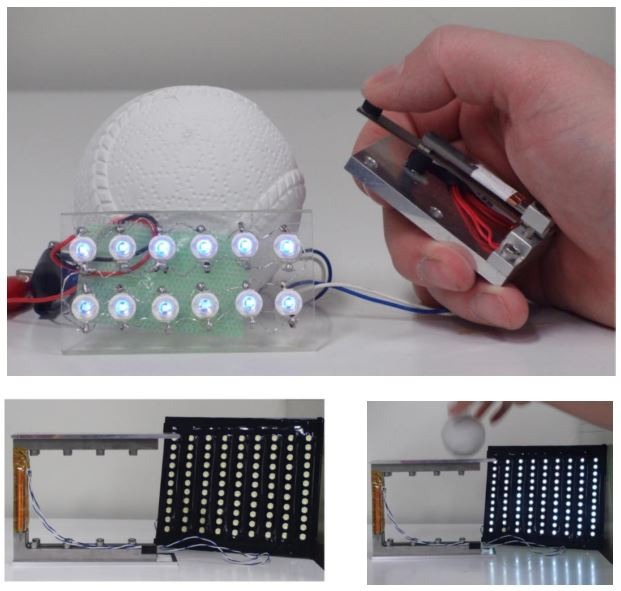
\includegraphics[width=0.5\textwidth]{energy-harvest-demo}
	\caption{Galfenol resonant beam energy harvester. Photo courtesy of Dr. Toshiyuki Ueno, Kanazawa University, Japan. Galfenol beams are in the same region as the coils and have dimensions of 3 mm thick x 15 mm width x 80 mm length.\cite{Slaughter2011}}
	\label{fig:energy-harvest-demo}
\end{figure}
The iron-based magnetostrictive alloy Fe-Ga (Galfenol, \fegacomp) is of interest for actuation, sensing and energy harvesting applications because in addition to its magnetostrictive properties, it is ductile and it has robust mechanical properties\cite{Clark2003}, relatively high permeability and good saturation magnetization (~1.7 T)\cite{Clark2002}. These properties allow our collaborator at Kanazawa University, Toshiyuki Ueno, to prototype highly-scalable Galfenol energy harvester devices with high efficiency, high power output, and low impedance\cite{Ueno2015a}, as seen in Figure \ref{fig:energy-harvest-demo}. Fe-Al (Alfenol, \fealcomp) has been overlooked as an actuactor because it has about half the magnetostriction of Fe-Ga alloys. However, Fe-Al has similar saturation magnetization ($\sim$1.5 T) and similar mechanical properties to Fe-Ga, making it an attractive energy harvester with the added benefit of being more earth abundant and less expensive than Fe-Ga\cite{Na2014a,Raghunath2014a}. 		

%TODO: get 3D figure of magnetic domains from Dr. Flatau
\begin{figure}[h]
	\centering
	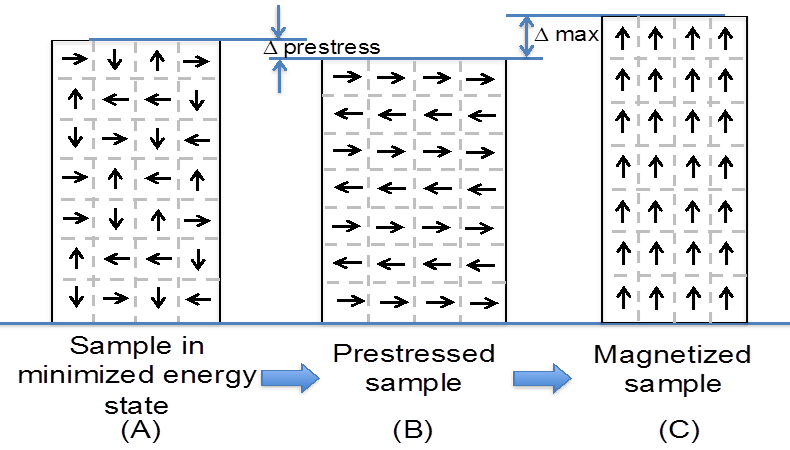
\includegraphics[width=0.5\textwidth]{prestressed-mag-anneal}
	\caption{Cartoons depicting a perfectly aligned cubic alloy with \hkl<100> magnetic easy axes as indicated. Arrows depict idealized orientation of magnetic domains.(A) Energy minimized state with closure domains randomly distributed throughout sample.  (B) Prestressed sample with aligned antiparallel magnetization vectors and sample length minimized due to stress-induced moment rotation. (C) Sample magnetized along length with $\Delta$max as the maximum achievable magnetostriction due to 90~$^{\circ}$ magnetic moment rotation.}
	\label{fig:prestressed-mag-anneal}
\end{figure}


Fe-Al is sufficiently magneto-elastic that coupling between bending stress and magnetic moment rotation yields readily observable time-varying magnetization changes in the alloy. In harvesters, power is generated in a copper coil that surrounds a magnetostrictive material when a time varying stress, e.g. vibration of the magnetostrictive material, produces a voltage in the coil (per Faraday’s law)\cite{Yoo2012}. Fe-Al is a body-centered cubic alloy textured to develop a  preferred orientation along the length of the strips by abnormal grain growth (AGG)\cite{Na2014,Na2014b,Na2013a}. The \hkl<100> directions are the magnetic easy axes. Subsequently, the stress annealing protocol was performed to introduce built-in uniaxial anisotropy perpendicular to the length of the strips\cite{Yoo2009}.  This was done to maximize 90$^{\circ}$ rotation of magnetic moments when the strip bends. Successful stress-anneal-induced magnetic anisotropy was achieved, but this stress annealing process could not provide uniform compressive stress on each tested sample leading to non-uniform magnetic flux change along the strip length. As a viable alternative for a uniform magnetic flux change, Brooks et al. have used magnetic field annealing to achieve nearly identical saturation magnetostriction under compressive and no preload values\cite{Brooks2012}. 



